\section{How place fields are detected: worked examples}
\label{sec:field_examples}
\noindent\textit{Analysis \texttt{field\_examples}, 38 sessions, fingerprint \texttt{6374297e80da}.}

The field counts and densities in the following sections all come from the procedure below (Fig.~\ref{fig:field_examples}; the cells shown are listed in Table~\ref{tab:field_examples:cells}).
\begin{enumerate}
\item \textbf{Linearisation.} Each position sample is projected onto the maze graph. Samples within 8\,cm of a node belong to that node's zone (96 zones); the rest fall into 4\,cm bins along the edges, giving 921 bins in total.
\item \textbf{Samples used.} Only samples inside trials with running speed $\geq 5$\,cm/s; units need $\geq 100$ spikes in those samples.
\item \textbf{Rate map.} Spike counts and occupancy per bin are each smoothed with a Gaussian of $\sigma = 5$\,cm over \emph{track} distance (no leak between neighbouring corridors) and divided. Bins with smoothed occupancy $< 0.3$\,s are invalid.
\item \textbf{Place cell.} Skaggs information above the null from 500 circular spike shifts ($\geq 20$\,s), $p < 0.05$, and at least one field.
\item \textbf{Field.} A connected set of valid bins with rate $\geq 30\%$ of \emph{that cell's} peak rate, with an in-field peak $\geq 1$\,Hz and a track extent $\geq 10$\,cm. The number of such sets is the cell's field count; a field's location is its peak bin.
\item \textbf{Surrogate.} The same steps on the cell's spikes after a circular shift in running time. Any field found there is produced by sampling noise alone.
\end{enumerate}

\begin{table}[htbp]
\centering
\scriptsize
\caption{Example cells of Fig.~\ref{fig:field_examples}.}
\label{tab:field_examples:cells}
\begin{tabular}{llrrrrrrrrrrr}
\toprule
rat & session & unit & pctl. & mean (Hz) & peak (Hz) & thr.\ (Hz) & SI & bins $\geq$ thr. & rejected & fields & median size (m) & surrogate fields \\
\midrule
Rat5 & GL2S5 & 407 & 10 & 0.503 & 15.5 & 4.64 & 1.28 & 10 & 0 & 2 & 0.263 & 13 \\
Rat5 & GL2S5 & 448 & 50 & 0.648 & 8.79 & 2.64 & 1.29 & 43 & 6 & 7 & 0.279 & 15 \\
Rat5 & GL2S5 & 457 & 90 & 1.83 & 10.4 & 3.12 & 0.354 & 155 & 32 & 25 & 0.199 & 26 \\
Rat6 & GL2S5 & 326 & 10 & 0.182 & 4.8 & 1.44 & 1.81 & 16 & 5 & 3 & 0.16 & 5 \\
Rat6 & GL2S5 & 13 & 50 & 2.39 & 23.7 & 7.12 & 1.26 & 84 & 7 & 13 & 0.315 & 3 \\
Rat6 & GL2S5 & 158 & 90 & 3.08 & 13.2 & 3.97 & 0.442 & 271 & 12 & 40 & 0.202 & 41 \\
\bottomrule
\end{tabular}
\end{table}

\begin{figure}[htbp]
\centering
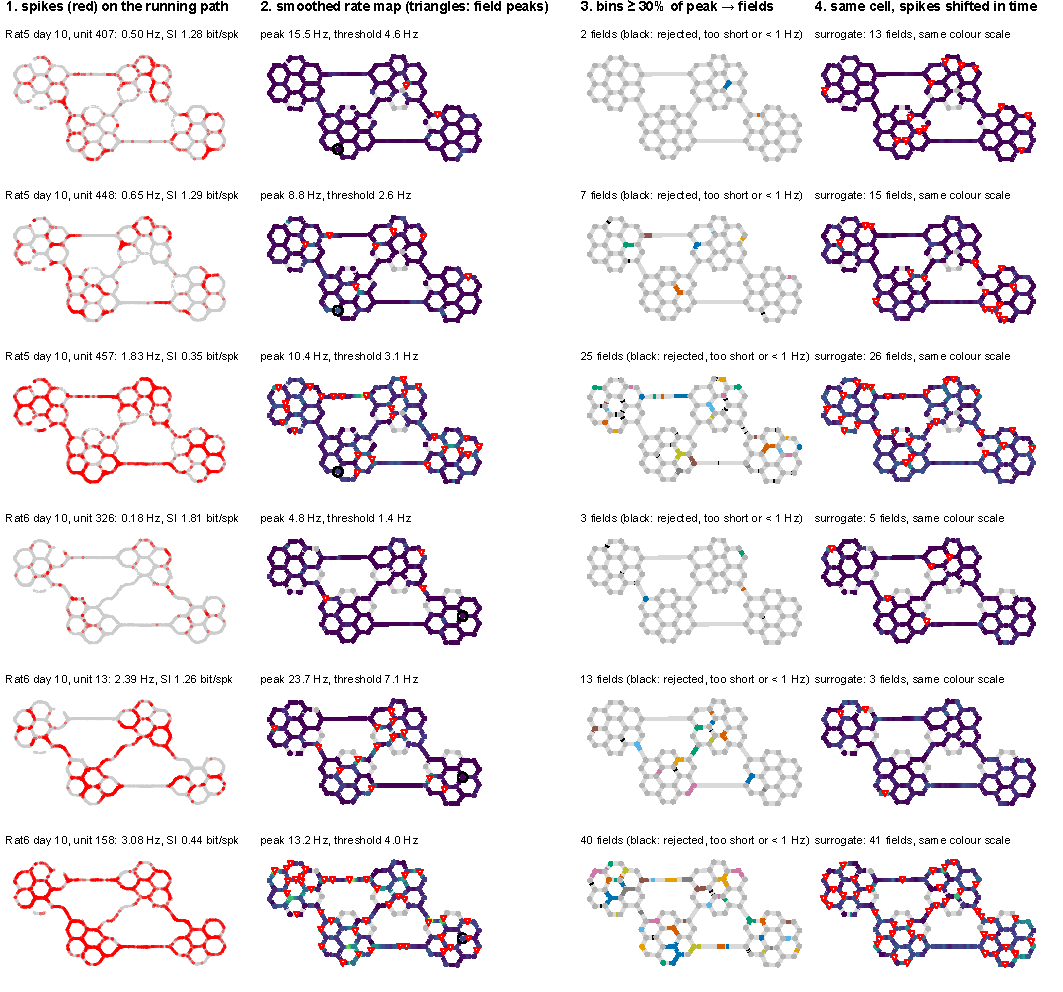
\includegraphics[width=\textwidth]{field_examples__field_examples.pdf}
\caption{\textbf{Field detection, step by step.} One mid-training session per rat (GL$n$S$x$: $x$-th session with the $n$-th goal location); rows are place cells at the 10th, 50th and 90th percentile of field count in that session. (1) Spikes emitted while running inside trials (red) on the animal's path (grey). (2) Rate map on the linearised maze, dark = 0, yellow = the cell's peak; open circle = goal node; triangles = peaks of accepted fields. (3) Bins at or above the threshold. Each connected group that passes the size and peak criteria is one field (colours repeat); black = above threshold but rejected; grey = below threshold or not visited.}
\label{fig:field_examples}
\end{figure}

\clearpage